\section{Our Method}
In this section, we first introduce the DU-Net after recapping the stacked U-Nets \cite{newell2016stacked}. Then we present the $order$-$K$ connectivity to improve its parameter efficiency, an efficient implementation to reduce its training memory,
and an iterative refinement to make it more parameter efficient.
% The skip blocks connecting the top-down and bottom-up blocks of the same spatial resolutions, are important to compensate the spatial information lost in the down-sampling of feature maps. 
Finally, network quantization is utilized to further reduce training memory and model size.
\subsection{DU-Net}
A U-Net contains top-down, bottom-up blocks and skip connections between them. Suppose multiple U-Nets are stacked together, for the $\ell^{th}$ top-down and bottom-up blocks in the $n^{th}$ U-Net, we use $f_\ell^n(\cdot)$ and $g_\ell^n(\cdot)$ to denote their non-linear transformations. Their outputs are represented by ${\bf x}_\ell^n$ and ${\bf y}_\ell^n$. $f_\ell^n(\cdot)$ and $g_\ell^n(\cdot)$ comprise operations of Convolution (Conv), Batch Normalization (BN) \cite{ioffe2015batch}, rectified linear units (ReLU) \cite{glorot2011deep}, and pooling.
% Besides, outputs of the $i^{th}$ top-down and bottom-up blocks in the $n^{th}$ U-Net are denoted by .
% For each block, we denote its input and output as $x$, $y$. Suppose multiple u-nets are stacked together, we use $x^{d_i}_\ell$, $x^{u_i}_\ell$ and $x^{s_i}_\ell$ to represent the inputs of the $i^{th}$ top-down, bottom-up and skip blocks in the $\ell^{th}$ u-net. Similar notations apply to $y$ and $z$.  

{\bf Stacked U-Nets.} The feature transitions at the $\ell^{th}$ top-down and bottom-up blocks of the $n^{th}$ U-Net are:

\begin{equation}\label{eq:hg}
    {\bf x}_\ell^n = f_\ell^n({\bf x}_{\ell-1}^n), {\bf y}_\ell^n = g_\ell^n({\bf y}_{\ell-1}^n+{\bf x}_\ell^n).
\end{equation}
The skip connections only exist locally within each U-Net, which may restrict that information flows across U-Nets.
% \[
%     x^{i+1}_{\ell}= 
% \begin{cases}
%     y^i_{\ell}, & \text{if } i \in TD\\
%      y^i_{\ell}+y^{(i+1)'}_\ell, & \text{elif } i \in BU
% \end{cases}
% \]
% \begin{equation}
%     y^i_\ell = \mathcal{F}^i_\ell([y^i_0,y^i_1,\cdots,y^i_{\ell-1},x^i_\ell])
% \end{equation}
% \begin{equation}
%     y_\ell = \mathcal{F}_\ell([y_0,y_1,\cdots,y_{\ell-1},x_\ell])
% \end{equation}

{\bf DU-Net.} To make information flow efficiently across stacked U-Nets, we propose a global connectivity pattern. Blocks at the same locations of different U-Nets have direct connections. Hence, we refer to this densely connected U-Nets architecture as {\it DU-Net}. Figure \ref{fig:framework} gives an illustration. Mathematically, the feature transitions at the $\ell^{th}$ top-down and bottom-up blocks of the $n^{th}$ U-Net can be formulated as:
\begin{equation}\label{eq:dense-inputs}
    {\bf x}_\ell^n = f_\ell^n([{\bf x}_{\ell-1}^n, {\bf X}_\ell^{n-1}]), {\bf y}_\ell^n = g_\ell^n([{\bf y}_{\ell-1}^n,{\bf x}_\ell^n,{\bf Y}_\ell^{n-1}]),
\end{equation}
where ${\bf X}_\ell^{n-1}={\bf x}_\ell^0,{\bf x}_\ell^1,\cdots,{\bf x}_\ell^{n-1}$ are the outputs of the $\ell^{th}$ top-down blocks in all preceding U-Nets. Similarly, ${\bf Y}_\ell^{n-1}={\bf y}_\ell^0,{\bf y}_\ell^1,\cdots,{\bf y}_\ell^{n-1}$ represent the outputs from the $\ell^{th}$ bottom-up blocks. $[\cdots]$ denotes the feature concatenation, which could make information flow more efficiently than the summation operation in Equation \ref{eq:hg}. 

According to Equation \ref{eq:dense-inputs}, a block receives features not only from connected blocks in the current U-Net but also the output features of the same semantic blocks from all its preceding U-Nets. Note that this semantic level dense connectivity is a generalization of the dense connectivity in DenseNet \cite{huang2016densely} that connects layers only within each block.

% at the semantic level by connecting the same semantic blocks in different U-Nets. In contrast
% $Order$-$1$ connectivity ({\bf Middle}) has connections not only for inputs of adjacent U-Nets (lower arrows), but also for their inside blocks (upper arrows). Similarly, $order$-$2$ connectivity ({\bf Bottom}) connects both inputs and inside blocks of 3 nearby U-Nets.
\begin{figure}[t]
\minipage[t]{0.49\textwidth}
\centering
  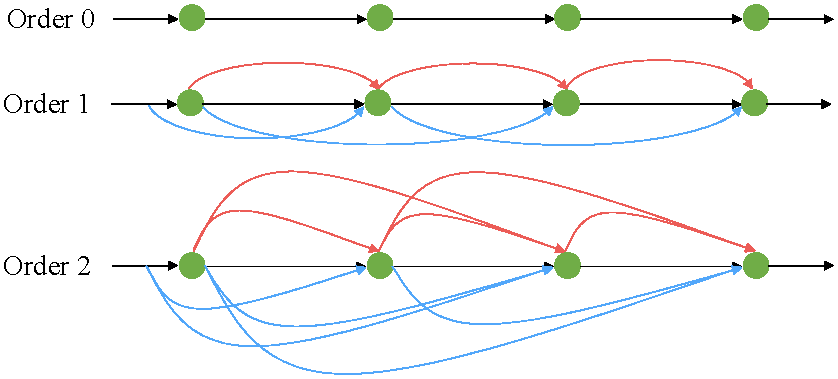
\includegraphics[width=0.9\linewidth]{figures/order-k-cropped.pdf}
%   \vspace*{-1mm}
  \caption{Illustration of $order$-$K$ connectivity. For simplicity, each dot represents one U-Net. The red and blue lines are the shortcut connections of inside semantic blocks and outside inputs. $Order$-$0$ connectivity ({\bf Top}) strings U-Nets together only by their inputs and outputs, i.e. stacked U-Nets. $Order$-$1$ connectivity ({\bf Middle}) has shortcut connections for adjacent U-Nets. Similarly, $order$-$2$ connectivity ({\bf Bottom}) has shortcut connections for 3 nearby U-Nets.}
\label{fig:$order$-$K$-illustr}
\endminipage \hfill
\minipage[t]{0.49\textwidth}
\centering
  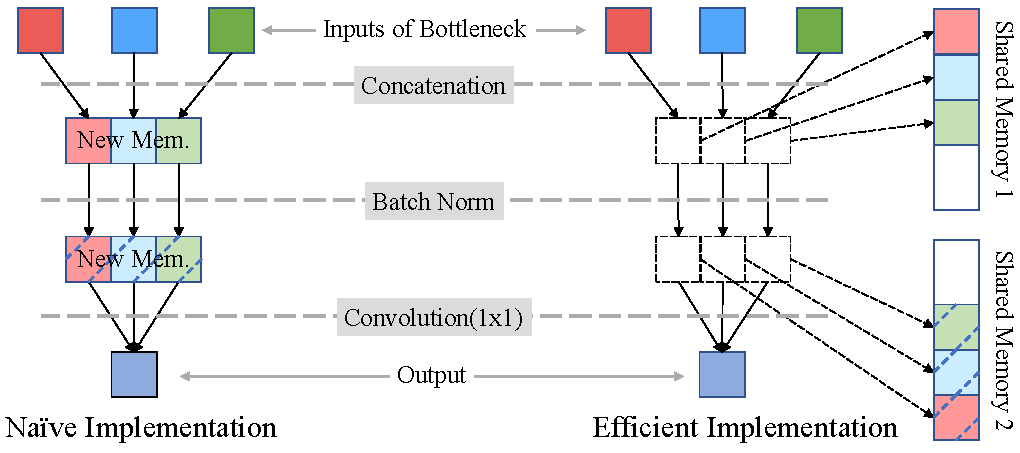
\includegraphics[width=0.9\linewidth]{figures/memory-efficient-cropped.pdf}
%   \vspace*{2mm}
  \caption{Illustration of memory efficient implementation. It is for the Concat-BN-ReLU-Conv($1\times 1$) in each bottleneck structure. ReLU is not shown since it is an inplace operation with no memory request. The efficient implementation  pre-allocates fixed memory space to store the concatenated and normalized features of connected blocks. In contrast, the naive implementation always allocates new memories for them, causing high memory consumption.}
  \label{fig:memory-efficient} \hfill
\endminipage
\end{figure}

% \begin{figure}[t!]
% \centering
%   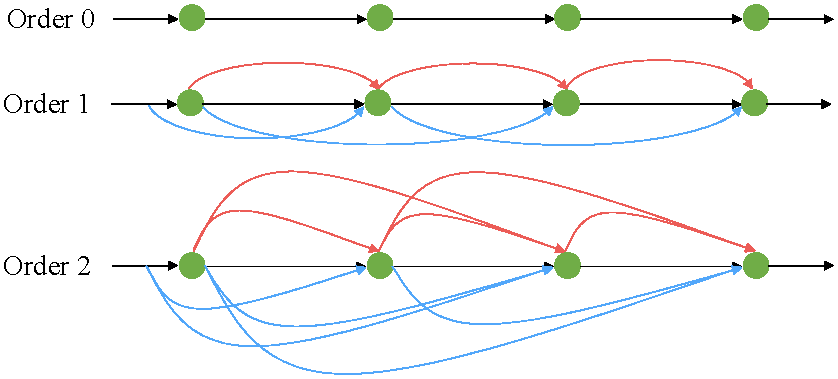
\includegraphics[width=.95\linewidth]{figures/order-k-cropped.pdf}
% \caption{Illustration of $order$-$K$ connectivity. For simplicity, each dot represents one U-Net. $Order$-$0$ connectivity ({\bf Top}) refers to that U-Nets are stringed together only by their inputs and outputs, i.e. stacked U-Nets. $Order$-$1$ connectivity ({\bf Middle}) has connections not only for inputs of adjacent U-Nets (lower arrows), but also for their inside blocks (upper arrows). Similarly, $order$-$2$ connectivity ({\bf Bottom}) connects both inputs and inside blocks of 3 nearby U-Nets.}
% \label{fig:$order$-$K$-illustr}
% \end{figure}

\subsection{${\bf Order}$-${\bf K}$ Connectivity}
In the above formulation of DU-Net, we connect blocks with the same semantic meanings across all U-Nets. The connections would have quadratic growth depth-wise. To make DU-Net parameter efficient, we propose to cut off some trivial connections. For compensation, we add an intermediate supervision at the end of each U-Net. The intermediate supervisions, as the skip connections, could also alleviate the gradient vanish problem. Mathematically, the features  ${\bf X}_\ell^{n-1}$ and ${\bf Y}_\ell^{n-1}$ in Equation \ref{eq:dense-inputs} turns into 
\begin{gather}
    {\bf X}_{\ell}^{n-1}={\bf x}_{\ell}^{n-k},\cdots,{\bf x}_{\ell}^{n-1},\\
    {\bf Y}_{\ell}^{n-1}={\bf y}_{\ell}^{n-k},\cdots,{\bf y}_{\ell}^{n-1},
\end{gather}
where $0\leq k\leq n$ represents how many preceding nearby U-Nets connect with the current one. $k=n$ or $k=0$ would result in the stacked U-Nets or fully densely connected U-Nets. A medium order could reduce the growth of DU-Net parameters from quadratic to linear. Therefore, it largely improves the parameter efficiency of DU-Net and could make DU-Net grow several times deeper.

The proposed $order$-$K$ connection has similar philosophy as the Variable Order Markov (VOM) models \cite{begleiter2004prediction}. Each U-Net can be viewed as a state in the Markov model. The current U-Net depends on a fixed number of preceding nearby U-Nets, instead of preceding either only one or all U-Nets. In this way, the long-range connections are cut off. Figure \ref{fig:$order$-$K$-illustr} illustrates connections of three different orders. In Figure \ref{fig:$order$-$K$-illustr}, the connections above the central axes follow VOM patterns of $order$-$0$, $order$-$1$ and $order$-$2$ whereas the central axes together with connections below them follow VOM patterns of $order$-$1$, $order$-$2$ and $order$-$3$.

Dense connectivity is a special case of $order$-$K$ connectivity on the limit of $K$. For small $K$, $order$-$K$ connectivity is much more parameter efficient. But fewer connections may affect the prediction accuracy of very deep DU-Net. To make DU-Net have both high parameter efficiency and prediction accuracy, we propose to use $order$-$K$ connectivity in conjunction with intermediate supervisions. In contrast, DenseNet \cite{huang2016densely} has only one supervision at the end. Thus, it cannot effectively take advantage of $order$-$K$ connectivity.
% It is worth pointing out that ${\bf Order}$-${\bf K}$ connectivity is a 
% $Y^{t}_{\ell-1}=y^{t}_{\ell-k},\cdots,y^{t}_{\ell-1}$.

% \begin{figure}[t!]
% \centering
%   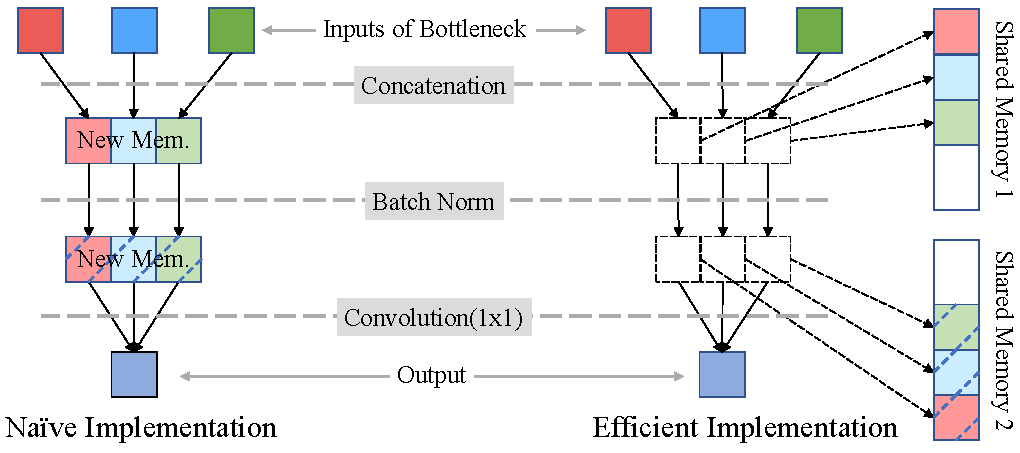
\includegraphics[width=.95\linewidth]{figures/memory-efficient-cropped.pdf}
% \caption{Illustration of memory efficient implementation. It is for the Concat-BN-ReLU-Conv($1\times 1$) in each bottleneck structure. ReLU is not shown since it is an inplace operation with no additional memory request. The efficient implementation  pre-allocates two fixed memory space to store the concatenated and normalized features of connected blocks. In contrast, the naive implementation always allocates new memories for them, causing high memory consumption.}
% \label{fig:memory-efficient}
% \end{figure}

\subsection{Memory Efficient Implementation}
% Compared with other existing network architectures, the DenseNet could achieve comparable performances with much fewer parameters, which benefits from its feature reuse. However, a naive implementation would make training large DenseNets expensive or even infeasible due to the quadratic growth of intermediate feature maps with respect to the depth. 
Benefitting from the $order$-$K$ connectivity, our DU-Net is quite parameter efficient. However, a naive implementation would prevent from training very deep DU-Net, since every connection would make a copy of input features. To reduce the training memory, we follow the efficient implementation \cite{pleiss2017memory}. More specifically, concatenation operations of the same semantic blocks in all U-Nets share a memory allocation and their subsequent batch norm operations share another memory allocation. Suppose a DU-Net includes $N$ U-Nets each of which has $L$ top-down blocks and $L$ bottom-up blocks. We need to pre-allocate two memory space for each of $2L$ semantic blocks. For the $\ell^{th}$ top-down blocks, the concatenated features $[{\bf x}_{\ell-1}^1, {\bf X}_\ell^0], \cdots, [{\bf x}_{\ell-1}^{N-1}, {\bf X}_\ell^{N-2}]$ share the same memory space. Similarly, the concatenated features $[{\bf y}_{\ell-1}^0,{\bf x}_\ell^0], [{\bf y}_{\ell-1}^1,{\bf x}_\ell^1,{\bf Y}_\ell^0], \cdots, [{\bf y}_{\ell-1}^{N-1},{\bf x}_\ell^{N-1},{\bf Y}_\ell^{N-2}]$ in the $\ell^{th}$ bottom-up blocks share the same memory space.

In one shared memory allocation, later produced features would overlay the former features. Thus, the concatenations and their subsequent batch norm operations require to be re-computed in backward phase. Figure \ref{fig:memory-efficient} illustrates naive and efficient implementations.

% \begin{figure*}[t!]
% \minipage{0.7\textwidth}
%     \centering
%   \includegraphics[width=0.95\linewidth]{figures/$order$-$K$-illustration-cropped.pdf}
% \endminipage
% \minipage{0.29\textwidth}
%     \centering
%   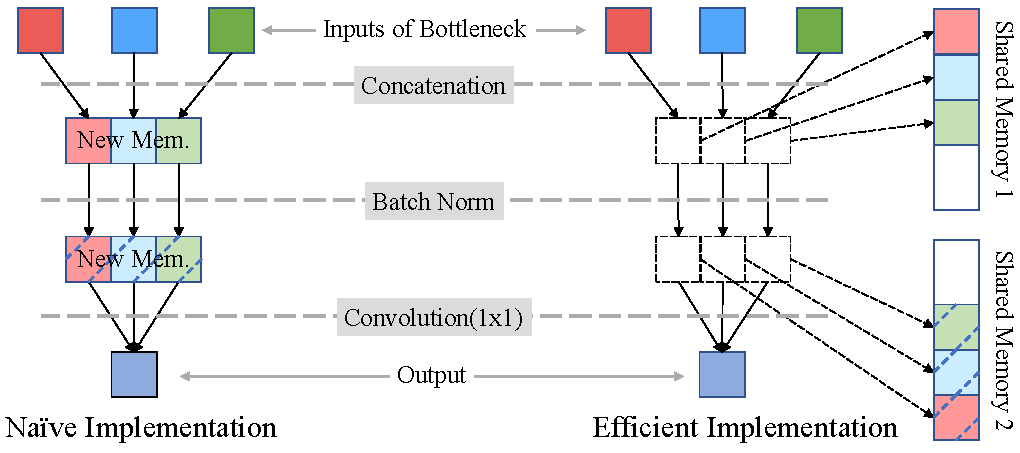
\includegraphics[width=0.99\linewidth]{figures/memory-efficient-cropped.pdf}
% \endminipage
% \caption{{\bf Left}: $order$-$K$ Connectivity. {\bf Right}: Memory Efficient Implementation.}
% \label{fig:overview}
% \end{figure*}


\subsection{Iterative Refinement}
In order to further improve the parameter efficiency of DU-Net, we consider an iterative refinement. It uses only half of a DU-Net but may achieve comparable performance. In the iterative refinement, a DU-Net has two forward passes. In the first pass, we concatenate the inputs of the first and last U-Nets and merge them in a small dense block. Then the refined input is fed forward in the DU-Net again. Better output is expected because of the refined input. 

In this iterative pipeline, the DU-Net has two groups of supervisions in the first and second iterations. Both the detection and regression supervisions \cite{bulat2016human} are already used in the landmark detection tasks. However, there is no investigation how they compare with each other. To this end, we could try different combinations of detection and regression supervisions for two iterations. Our comparison could give some guidance for future research. 
% \begin{figure}[hbt]
% \centering
%   \includegraphics[width=\linewidth]{figures/iteration-cropped.pdf}
% \caption{}
% \label{fig:iteration}
% \end{figure}
% To further improve the prediction accuracy of DU-Net, we use some feature maps near its output to refine its original input. An illustration is given in Figure \ref{}.

%G%
\subsection{Network Quantization}

We aim at cutting down high precision operations and parameters both in training and inference stages of DU-Net. The bit-width of weights can be reduced to one or two bits through sign function or symmetrical threshold, whereas the layerwise gradients and inputs are quantized with linear mapping. In previous XNOR-Net \cite{rastegari2016xnor}, a scaling factor was introduced to approximate the real-value weight. However, calculating these float factor costs additional computational resources. To further decrease memory usage and model size, we try to remove the scaling factor and follow WAGE \cite{wu2018training} to quantize dataflow during training. More specifically, weights are binarized to -1 and 1 by the following equation:
\begin{equation} \label{eq:sign}
q(x) = sign(clip(x,-1,1))
\end{equation} 
or ternarized to -1, 0 and -1 by the a positive threshold $\delta$ as \cite{li2016ternary} presented, where $\delta \approx \frac{0.7}{n}\sum_{i=1}^{n} \left | w_i \right |$ provided that $w_i$ is initialized by Gaussian distributions. The dataflows, i.e. gradients and inputs, are quantized to $k$-bit values by the following linear mapping function:
\begin{equation} \label{eq:sign}
q(x,k) = clip(\sigma(k)\cdot  round(x\sigma(k)) -1+\sigma(k),1-\sigma(k))
\end{equation} 
Here, the unit distance $\sigma$ is calculated by $\sigma(k) = \frac{1}{2^{k-1}}$. In the following experiments, we explore different combinations of bit-widths to balance performance and memory consumption.
%G%
